\section{Esercizio 1 -- Multiplexer 16:1}
\subsection{Esercizio 1.1}
Per la risoluzione dell’esercizio, è stato adottato un approccio modulare, scomponendo la macchina da implementare in componenti più piccoli e integrandoli progressivamente fino all'implementazione finale del multiplexer indirizzabile 16:1. Seguendo le specifiche della traccia, il multiplexer 16:1 è stato realizzato attraverso la composizione di cinque multiplexer 4:1 [Figura \ref{fig:mux_4_1}].

\begin{figure}[h]
    \centering
    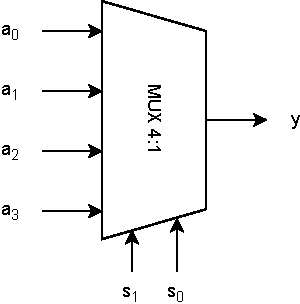
\includegraphics[width=0.25\textwidth]{img/mux_4_1.pdf}
    \caption{Architettura del multiplexer 4:1}
    \label{fig:mux_4_1}
\end{figure}

Il circuito risultante dispone di 16 ingressi e un’unica uscita. Trattandosi di un multiplexer indirizzabile, sono previsti quattro ulteriori ingressi di selezione, che determinano quale dei 16 segnali di ingresso viene trasmesso in uscita [Figura \ref{fig:mux_16_1}].

\begin{figure}[h]
    \centering
    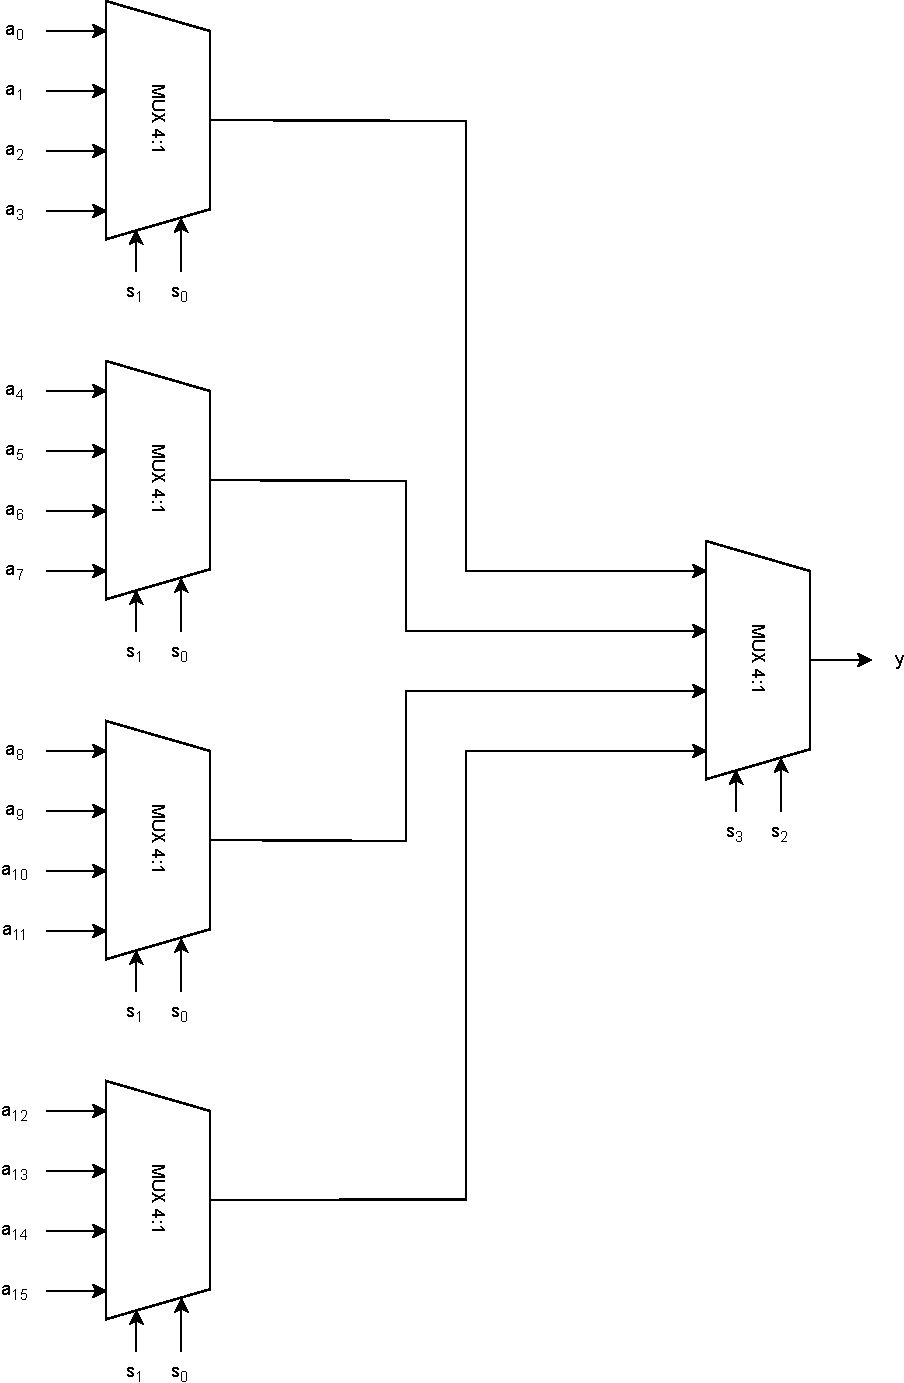
\includegraphics[width=0.4\textwidth]{img/mux_16_1.pdf}
    \caption{Architettura del multiplexer 16:1}
    \label{fig:mux_16_1}
\end{figure}

Come anticipato, il multiplexer 16:1 è stato realizzato mediante la composizione di cinque multiplexer 4:1.

I primi quattro multiplexer 4:1 ricevono ciascuno un gruppo di quattro ingressi tra i 16 totali del multiplexer 16:1. Utilizzando i primi due segnali di selezione ($s_1$ ed $s_0$), ciascuno di essi genera un'uscita, riducendo così il numero di segnali a quattro.

Queste quattro uscite diventano gli ingressi del quinto multiplexer 4:1, il quale, tramite i restanti segnali di selezione $s_3$ e $s_2$, determina l'uscita finale $y$ [Figura \ref{fig:1_1_MUX_16_1}].

\begin{figure}[h]
    \centering
    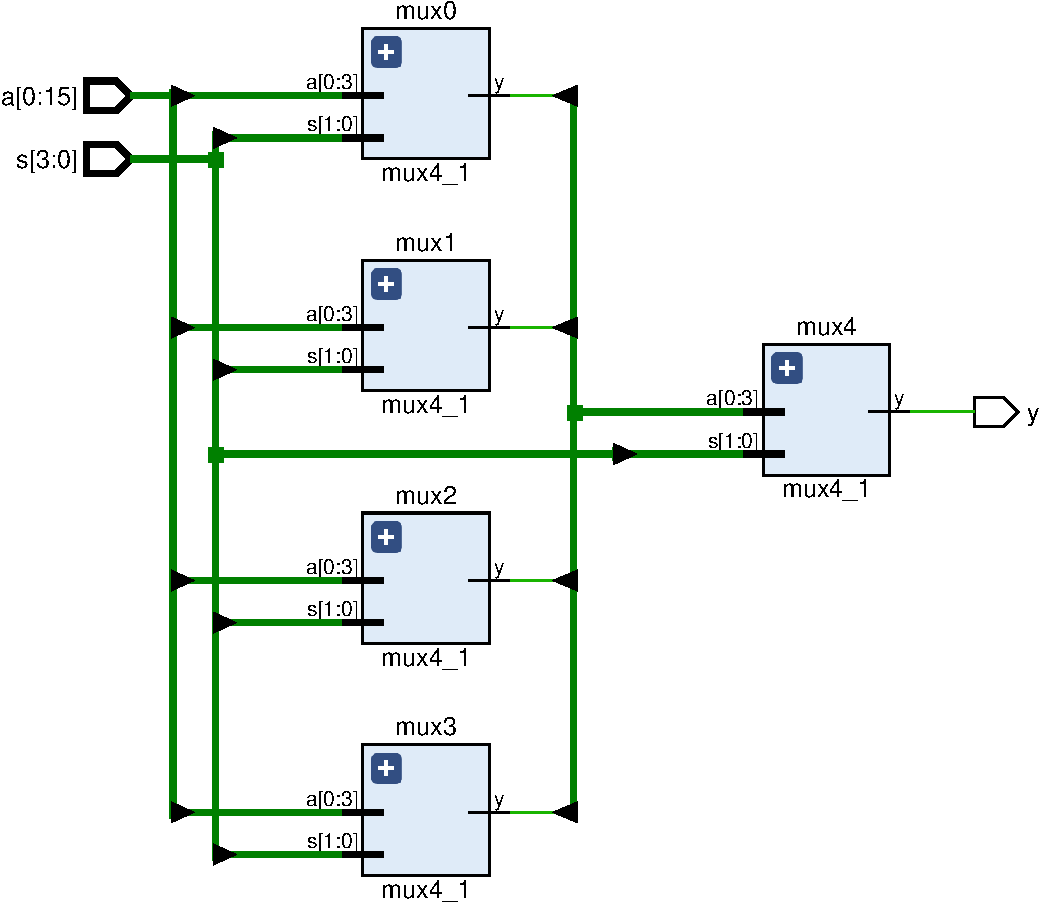
\includegraphics[width=0.6\textwidth]{img/1_1_MUX_16_1.pdf}
    \caption{Schema a blocchi del progetto}
    \label{fig:1_1_MUX_16_1}
\end{figure}

\subsubsection{Implementazione}
Il mux 16:1 ha un comportamento quasi analogo a quello del mux 4:1, con unica differenza il numero di segnali di ingresso, e di conseguenza il numero di segnali di selezione (si veda [Codice sorgente \ref{cod:mux_4_1}] per mux 4:1).

\begin{code}
    \inputminted{vhdl}{vhdl/mux16_1.vhd}
    \caption{Implementazione del multiplexer 16:1}
    \label{cod:mux16_1}
\end{code}

Inizialmente, si è definita l’entità \texttt{mux16\_1}, specificando i 16 ingressi, i 4 bit di selezione e l’uscita. Questa entità non è implementata direttamente come un unico blocco, ma viene costruita assemblando multiplexer 4:1, ciascuno dei quali seleziona uno tra 4 ingressi in base a 2 bit di selezione.

L’architettura scelta è di tipo \texttt{structural} [Codice sorgente \ref{cod:mux16_1}], cioè organizziamo il circuito collegando tra loro componenti più piccoli. Per farlo, si è dichiarato il componente \texttt{mux4\_1}, che rappresenta un multiplexer con 4 ingressi, 2 bit di selezione e 1 uscita. Questo componente viene poi utilizzato più volte per realizzare il multiplexer 16:1.

La logica del circuito si sviluppa in due livelli:

\begin{enumerate}
    \item Primo livello: I primi 4 multiplexer 4:1 ricevono gruppi di 4 bit ciascuno dagli ingressi principali e utilizzano i 2 bit meno significativi di selezione (\texttt{s(1 downto 0)}) per scegliere quale dei 4 ingressi trasmettere in uscita. Questo genera 4 uscite intermedie, memorizzate in un segnale temporaneo \texttt{u}.
    \item Secondo livello: Un quinto multiplexer 4:1 riceve in ingresso i 4 segnali intermedi e utilizza i 2 bit più significativi di selezione (\texttt{s(3 downto 2)}) per scegliere quale inviare all’uscita finale \texttt{y}.
\end{enumerate}

Grazie a questa struttura, il multiplexer 16:1 è in grado di selezionare qualunque ingresso tra i 16 disponibili, sfruttando in modo efficiente i 4 bit di selezione. Questo approccio modulare permette di suddividere il problema in sotto-componenti più semplici e facilmente riutilizzabili, garantendo un design ordinato e scalabile.

\subsubsection{Simulazione}
Per effettuare la simulazione il primo passo da compiere è la stesura del testbench. Prima di discutere quanto fatto è bene osservare il codice:

\begin{code}
    \inputminted{vhdl}{vhdl/mux16_1_tb.vhd}
    \caption{Testbench del multiplexer 16:1}
    \label{cod:mux16_1_tb}
\end{code}

La prima operazione svolta è stata la dichiarazione di un’entity. Si può notare che il corpo dell’entity è vuoto, poiché il testbench non rappresenta un componente hardware da implementare, ma serve esclusivamente per la simulazione e la verifica del corretto funzionamento del sistema.

Un testbench non ha segnali di ingresso o uscita perché non viene istanziato da altri blocchi, ma al contrario, è lui a istanziare il componente da testare. In questo caso, il nostro Unit Under Test (\texttt{uut}) è il multiplexer 16:1, che viene collegato a segnali di test tramite il port map.

Prima dell’istanza del uut, vengono dichiarati i segnali necessari alla simulazione:

\begin{itemize}
    \item \texttt{input}, che rappresenta i 16 ingressi del multiplexer.
    \item \texttt{control}, il vettore di selezione a 4 bit.
    \item \texttt{output}, l’uscita del multiplexer.
\end{itemize}

Infine, è stato definito un process di stimolazione (\texttt{stim\_process}), che ha il compito di fornire diversi valori di input al multiplexer e verificare che l’uscita corrisponda al valore atteso. In questo modo, possiamo validare il corretto funzionamento del sistema [Figura \ref{fig:mux16_1_tb}].

\begin{figure}[h]
    \centering
    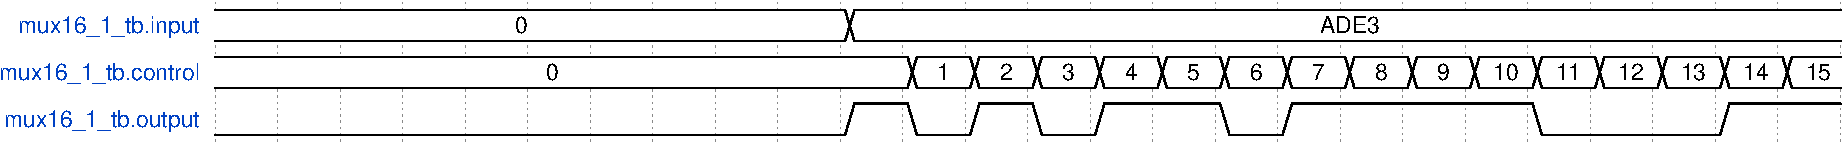
\includegraphics[width=\textwidth]{img/mux16_1_tb.pdf}
    \caption{Simulazione del multiplexer 16:1}
    \label{fig:mux16_1_tb}
\end{figure}

\subsection{Esercizio 1.2}
Per la risoluzione dell'esercizio di progettazione della rete di interconnessione, si è adottato un approccio modulare, suddividendo il problema in componenti più piccoli per semplificare l'implementazione complessiva. In particolare, l'implementazione coinvolge due componenti principali: un multiplexer 16:1 e un demultiplexer 1:4 (si veda [Codice sorgente \ref{cod:dmux_1_4}] per dmux 1:4) [Figure \ref{fig:interconnection16_4}, \ref{fig:1_2_INTERCONNECTION_16_4}].

\begin{figure}[h]
    \centering
    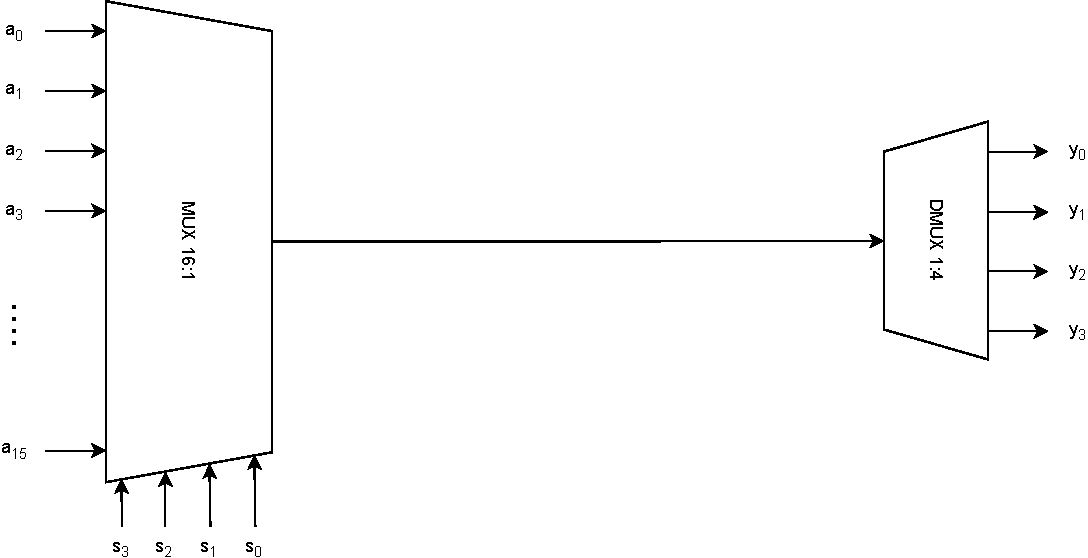
\includegraphics[width=0.6\textwidth]{img/interconnection16_4.pdf}
    \caption{Architettura dell'interconnessione 16:4}
    \label{fig:interconnection16_4}
\end{figure}

\begin{figure}[h]
    \centering
    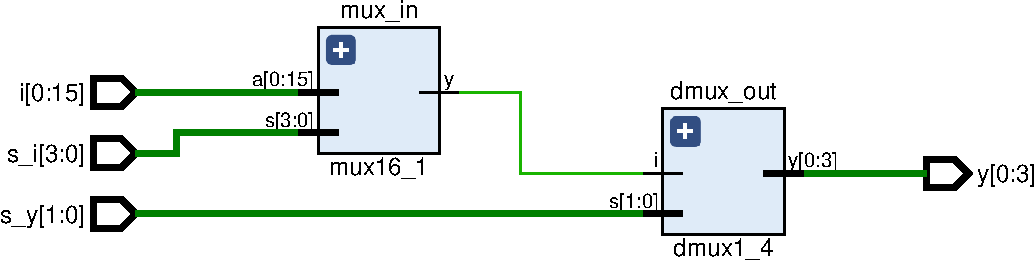
\includegraphics[width=0.6\textwidth]{img/1_2_INTERCONNECTION_16_4.pdf}
    \caption{Schema a blocchi del progetto}
    \label{fig:1_2_INTERCONNECTION_16_4}
\end{figure}

\subsubsection{Implementazione}
\begin{code}
    \inputminted{vhdl}{vhdl/interconnection16_4.vhd}
    \caption{Implementazione dell'interconnessione 16:4}
    \label{cod:interconnection16_4}
\end{code}

Questo codice VHDL implementa un sistema di interconnessione 16:4, che permette di selezionare una delle 16 linee di ingresso e distribuirne il valore su una delle 4 linee di uscita.

Il codice è organizzato in maniera modulare, sfruttando due componenti esterni:

\begin{itemize}
    \item \texttt{mux16\_1}: un multiplexer 16:1 che seleziona uno tra 16 segnali di ingresso.
    \item \texttt{dmux1\_4}: un demultiplexer 1:4 che invia il segnale ricevuto a una delle 4 linee di uscita.
\end{itemize}

L’architettura è dichiarata come \texttt{structural} [Codice sorgente \ref{cod:interconnection16_4}], il che significa che il circuito è costruito collegando tra loro componenti più piccoli. Inoltre, viene dichiarato un segnale intermedio (interconnection), che funge da collegamento tra il multiplexer e il demultiplexer.

Il multiplexer \texttt{mux16\_1} riceve i 16 ingressi (\texttt{i}) e, in base ai 4 bit di selezione \texttt{s\_i}, sceglie uno solo di essi, che viene trasmesso sul segnale interconnection. Il valore selezionato viene poi passato al demultiplexer \texttt{dmux1\_4}, che, in base ai 2 bit di selezione \texttt{s\_y}, lo indirizza su una delle 4 uscite \texttt{y}, mentre le altre uscite rimangono a zero.

In altre parole, il sistema permette di scegliere un ingresso tra 16 disponibili e di inviarlo a una delle 4 uscite disponibili, creando così una connessione dinamica tra ingresso e uscita.

\subsubsection{Simulazione}
Per effettuare la simulazione il primo passo da compiere è la stesura del testbench. Prima di discutere quanto fatto è bene osservare il codice in figura:

\begin{code}
    \inputminted{vhdl}{vhdl/interconnection16_4_tb.vhd}
    \caption{Testbench dell'interconnessione 16:4}
    \label{cod:interconnection16_4_tb}
\end{code}

Il suo obiettivo principale è controllare se il circuito seleziona correttamente un ingresso tra i 16 disponibili e lo instrada in modo adeguato su una delle 4 uscite. Per prima cosa, il testbench dichiara l’entità \texttt{interconnection16\_4\_tb}. Essendo un testbench, questa entità non ha porte di ingresso o uscita, perché il suo compito non è quello di rappresentare un vero e proprio circuito, ma di simulare il comportamento del sistema che vogliamo testare.

All’interno dell’architettura \texttt{behavioral}, viene dichiarato e istanziato il componente da testare, cioè \texttt{interconnection16\_4}. Per poter effettuare i test, vengono poi definiti alcuni segnali di simulazione che sostituiscono gli ingressi e le uscite del circuito reale. In particolare:

\begin{itemize}
    \item \texttt{input}: un vettore di 16 bit che rappresenta gli ingressi del sistema.
    \item \texttt{control\_input}: un segnale di 4 bit che serve a selezionare quale ingresso utilizzare.
    \item \texttt{output}: un vettore di 4 bit che rappresenta le possibili uscite del circuito.
    \item \texttt{control\_output}: un segnale di 2 bit che stabilisce su quale uscita il segnale selezionato verrà instradato.
\end{itemize}

Successivamente, il componente \texttt{interconnection16\_4} viene collegato a questi segnali attraverso un port map, che permette di simulare il suo comportamento all’interno del testbench. La parte più importante del codice è il processo di stimolazione \texttt{stim\_proc}, che ha il compito di generare i segnali di ingresso e verificare che le uscite siano corrette [Figura \ref{fig:interconnection16_4_tb}].

\begin{figure}[h]
    \centering
    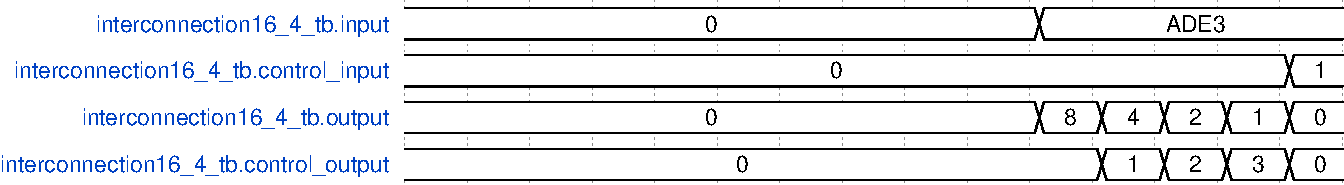
\includegraphics[width=\textwidth]{img/interconnection16_4_tb.pdf}
    \caption{Simulazione dell'interconnessione 16:4}
    \label{fig:interconnection16_4_tb}
\end{figure}

\subsection{Esercizio 1.3}
Per implementare su board il progetto della rete di interconnessione ci si è focalizzati su due componenti principali: l’unità di controllo e la rete di interconnessione 16:4. L'obiettivo è implementare una rete di interconnessione 16:4 su una FPGA, utilizzando switch e pulsanti come input e LED per visualizzare l'output.

\begin{code}
    \inputminted{vhdl}{vhdl/interconnection16_4_control_unit.vhd}
    \caption{Implementazione dell'unità di controllo}
    \label{cod:interconnection16_4_control_unit}
\end{code}

Il codice VHDL definisce un'unità di controllo \texttt{control\_unit}, che gestisce il caricamento di dati in un registro a 16 bit, suddiviso in due parti da 8 bit ciascuna. Il funzionamento di questa unità è sincronizzato con un segnale di clock, quindi i dati vengono aggiornati solo al fronte di salita del clock (quando passa da 0 a 1).

L’entità \texttt{control\_unit} ha diversi segnali di ingresso e uscita:

\begin{itemize}
    \item \texttt{clock}: segnale di clock per sincronizzare l'aggiornamento dei dati.
    \item \texttt{load\_first\_part}, \texttt{load\_second\_part}: segnali di controllo per indicare quale parte del registro deve essere aggiornata.
    \item \texttt{bits\_in}: vettore di 8 bit che contiene il valore da caricare.
    \item \texttt{bits\_out}: vettore di 16 bit che rappresenta il registro interno aggiornato.
\end{itemize}

All’interno dell’architettura \texttt{behavioral} [Codice sorgente \ref{cod:interconnection16_4_control_unit}], viene dichiarato un segnale \texttt{input}, inizializzato a zero, che funge da registro interno per memorizzare i dati. Questo segnale viene poi assegnato direttamente all'uscita \texttt{bits\_out}, in modo che l’uscita rifletta sempre lo stato attuale del registro.

Il cuore del codice è un processo sensibile al segnale di clock. Questo significa che il processo viene eseguito ogni volta che il clock cambia stato.
All’interno del processo:

\begin{itemize}
    \item Si verifica \texttt{clock'event and clock = `1'}, ossia il verificarsi di un evento sul clock quando passa da 0 a 1, per garantire che il caricamento dei dati avvenga solo sul fronte di salita.
    \item Si controlla quale parte del registro aggiornare:
          \begin{itemize}
              \item Se \texttt{load\_first\_part = `1'}, il valore presente in \texttt{bits\_in} viene copiato nei primi 8 bit (\texttt{0 to 7}) del registro.
              \item Se \texttt{load\_second\_part = `1'}, \texttt{bits\_in} viene copiato negli ultimi 8 bit (\texttt{8 to 15}) del registro.
          \end{itemize}
    \item Se entrambi i segnali di controllo sono a `0', il contenuto del registro rimane invariato.
\end{itemize}

\begin{code}
    \inputminted{vhdl}{vhdl/interconnection16_4_onboard.vhd}
    \caption{Implementazione dell'interconnessione 16:4 su board}
    \label{cod:interconnection16_4_onboard}
\end{code}

L’obiettivo è permettere all’utente di caricare un dato di 16 bit utilizzando 8 switch alla volta e poi selezionare quale bit trasmettere in uscita attraverso una rete di multiplexer e demultiplexer.

\begin{enumerate}
    \item Caricamento del dato in ingresso (16 bit totali). Gli 8 switch di sinistra (\texttt{SW\_DATA}) servono per inserire i dati:
          \begin{itemize}
              \item Premendo \texttt{BTNL}, i primi 8 bit vengono caricati nei registri di ingresso.
              \item Premendo \texttt{BTNR}, vengono caricati i secondi 8 bit.
          \end{itemize}
    \item Selezione del bit di ingresso e della linea di uscita. Gli switch di destra (\texttt{SW\_SEL}) servono per selezionare i dati:
          \begin{itemize}
              \item I primi 4 bit (\texttt{SW\_SEL(5 downto 2)}) scelgono quale dei 16 bit inviare in uscita.
              \item Gli ultimi 2 bit (\texttt{SW\_SEL(1 downto 0)}) determinano su quale LED far comparire il bit selezionato.
          \end{itemize}
    \item Visualizzazione dell’output. Il risultato viene mostrato sui 4 LED più a sinistra (\texttt{LED(15 downto 12)}).
\end{enumerate}

La dichiarazione dell’entità \texttt{interconnection16\_4\_onboard} definisce i segnali di input e output della rete di interconnessione, mentre nella dichiarazione dei componenti utilizzati, ritroviamo la \texttt{control\_unit}, che gestisce il caricamento degli 8 bit alla volta nel registro di ingresso da 16 bit e la \texttt{interconnection16\_4}, che contiene il multiplexer 16:1 per selezionare un bit di ingresso e il demultiplexer 1:4 per distribuire il bit su uno dei 4 LED.

Per poter utilizzare la board è stato necessario effettuare alcune modifiche al file dei constraints \texttt{Nexys A7-100T-Master.xdc}. In particolare, abbiamo dovuto aggiungere i seguenti vincoli:
\begin{itemize}
    \item Abilitare il clock a 100 MHz.
    \item Abilitare gli switch \texttt{SW0}--\texttt{SW5} e \texttt{SW8}--\texttt{SW15} per l’input.
    \item Abilitare i pulsanti \texttt{BTNL} e \texttt{BTNR} per il controllo del caricamento dei dati.
    \item Abilitare i LED \texttt{LED15}--\texttt{LED12} per la visualizzazione dell’output.
\end{itemize}
